\chapter{第二章 理论基础}
\section{预训练大模型概述}
近年来,预训练大模型(Large Pretrained Models, LPMs)在自然语言处理(NLP)领域取得了突破性进展。这些模型,如 GPT-4、T5 和 BERT,凭借其强大的语言理解和生成能力,正在改变我们处理文本数据的方式。这些模型通常在海量的文本数据上进行无监督预训练,通过学习语言的深层语义关系,能够捕捉到复杂的语言模式和结构。预训练完成后,这些模型可以通过有监督的微调来适应各种特定的自然语言处理任务,如文本分类、机器翻译、问答系统等。

在智能驾驶场景生成领域,预训练大模型的应用具有重要意义。传统的场景生成方法通常依赖于手工编写规则或模板,这些方法虽然在一定程度上能够生成有效的场景,但存在效率低下、灵活性差和难以扩展等问题。预训练大模型的引入极大地提升了自然语言指令理解的精度与灵活性,能够将模糊的自然语言描述自动映射为结构化的场景代码。与传统的规则模板方法相比,基于大模型的方法能够适应更复杂、多样的用户输入,具有更强的泛化能力和鲁棒性。

本项目基于开放领域大模型(如 OpenAI 的 GPT 系列),针对智能驾驶场景描述进行定向设计。通过微调这些模型,使其能够直接生成符合 Scenic 语法规范的场景定义脚本,为后续的仿真与评估提供输入支持。这种基于大模型的方法不仅提高了场景生成的效率,还能够生成更具创新性和多样性的场景,为自动驾驶技术的研发和测试提供了更强大的工具。

\section{自然语言场景建模}
自然语言场景建模(Natural Language-based Scenario Modeling)是将人类用自然语言描述的复杂交通场景转化为机器可理解的格式的过程。这一过程是智能驾驶场景生成的关键步骤,因为它直接决定了生成场景的质量和可用性。在本研究中,目标是将自然语言直接映射为 Scenic 脚本代码,从而实现从自然语言描述到可执行仿真场景的无缝转换。

常见的自然语言场景建模方法包括:
\begin{itemize}
	\item \textbf{检索式建模(Retrieval-Based Modeling)}:这种方法通过从已有场景数据库中检索与输入描述最相似的场景来生成新的场景。检索式建模的优点是能够快速生成与已有场景相似的新场景,但其局限性在于依赖于数据库中的已有场景,无法生成全新的场景。
	\item \textbf{生成式建模(Generative Modeling)}:这种方法通过预训练语言模型直接生成场景脚本。生成式建模的优点是能够生成全新的场景,具有更高的创新性和多样性。然而,生成式建模的挑战在于如何确保生成的场景符合实际的交通规则和逻辑。
	\item \textbf{检索与生成结合(Retrieve-then-Generate)}:这种方法结合了检索式建模和生成式建模的优点,先从数据库中检索相关的场景,然后基于检索结果生成新的场景。这种方法能够在保持生成多样性的同时,利用已有场景的结构和逻辑。
\end{itemize}

在 ChatScene 项目中,采用的是检索式建模,通过 sentence-transformers/sentence-t5-large 模型对场景描述进行向量化,基于相似度检索最接近的场景模板。这种方法虽然能够快速生成场景,但其生成能力受限于数据库的规模和覆盖范围。为了突破检索方式的局限,本项目进一步引入生成式大模型,实现 end-to-end 场景生成,从而提升场景的创新性与多样性。

\section{Scenic 场景描述语言}
Scenic 是一种为智能驾驶仿真而设计的专用场景描述语言(Domain-Specific Language, DSL)。它通过简洁而强大的语法,允许用户定义车辆、道路、行人等元素在仿真环境中的属性与关系。Scenic 的主要特点包括:
\begin{itemize}
	\item \textbf{声明式语法(Declarative Syntax)}:Scenic 采用声明式语法,用户可以通过简单直观的语句描述对象的位置、朝向、速度等属性。这种语法使得场景定义更加直观和易于理解。
	\item \textbf{支持不确定性(Probabilistic Support)}:Scenic 允许定义位置、角度、速度等属性的概率分布,从而能够生成更加多样化的场景。这种不确定性支持使得生成的场景更加接近真实世界的复杂性和随机性。
	\item \textbf{易于与仿真器集成(Integration-Friendly)}:Scenic 可以直接导出到 CARLA、LGSVL 等主流仿真平台,使得生成的场景能够快速用于自动驾驶系统的测试和验证。
\end{itemize}

在本项目中,预训练大模型需要生成符合 Scenic 语法的代码。因此,理解 Scenic 的基本结构和表达方式是实现自然语言到场景生成系统的关键基础。通过将自然语言描述转换为 Scenic 脚本,我们能够将人类的直观描述转化为机器可执行的仿真场景,从而为自动驾驶技术的研发和测试提供强大的支持。

\section{智能驾驶仿真平台 CARLA}
CARLA(Car Learning to Act)是目前应用最广泛的开源自动驾驶仿真平台之一。它提供了丰富的城市场景、传感器模拟、车辆动力学建模与环境交互能力,使得研究人员能够在虚拟环境中测试和验证自动驾驶系统。CARLA 的主要特点包括:
\begin{itemize}
	\item \textbf{高度可定制的地图与交通要素}:CARLA 允许用户自定义地图和交通要素,从而能够模拟各种复杂的交通场景。
	\item \textbf{多种传感器模拟}:CARLA 支持多种传感器模拟,包括 RGB 相机、LiDAR、雷达等,使得研究人员能够测试自动驾驶系统在不同传感器配置下的表现。
	\item \textbf{支持复杂行为建模与自动驾驶决策系统测试}:CARLA 提供了强大的行为建模工具,使得研究人员能够模拟各种复杂的交通行为和自动驾驶决策系统。
\end{itemize}
本项目采用 CARLA 0.9.15 版本作为仿真环境。通过将生成的 Scenic 脚本转译成 CARLA 可执行场景,我们能够实现自然语言指令到仿真测试的完整闭环。这种从自然语言描述到仿真测试的无缝转换,为自动驾驶技术的研发和测试提供了一种高效、灵活的方法。

\section{ChatScene 项目基础与本项目创新点}
ChatScene 是近期提出的一套基于知识检索的安全关键场景生成系统。它主要通过使用 sentence-t5-large 模型对自然语言描述进行检索匹配,结合 SafeBench 框架在 CARLA 上进行仿真测试。ChatScene 的主要思路是利用已有的场景数据库,通过检索与输入描述最相似的场景来生成新的场景。这种方法的优点是能够快速生成与已有场景相似的新场景,但其局限性在于依赖于数据库中的已有场景,无法生成全新的场景。它的整体结构如下:
\begin{figure}[H]
	\centering
	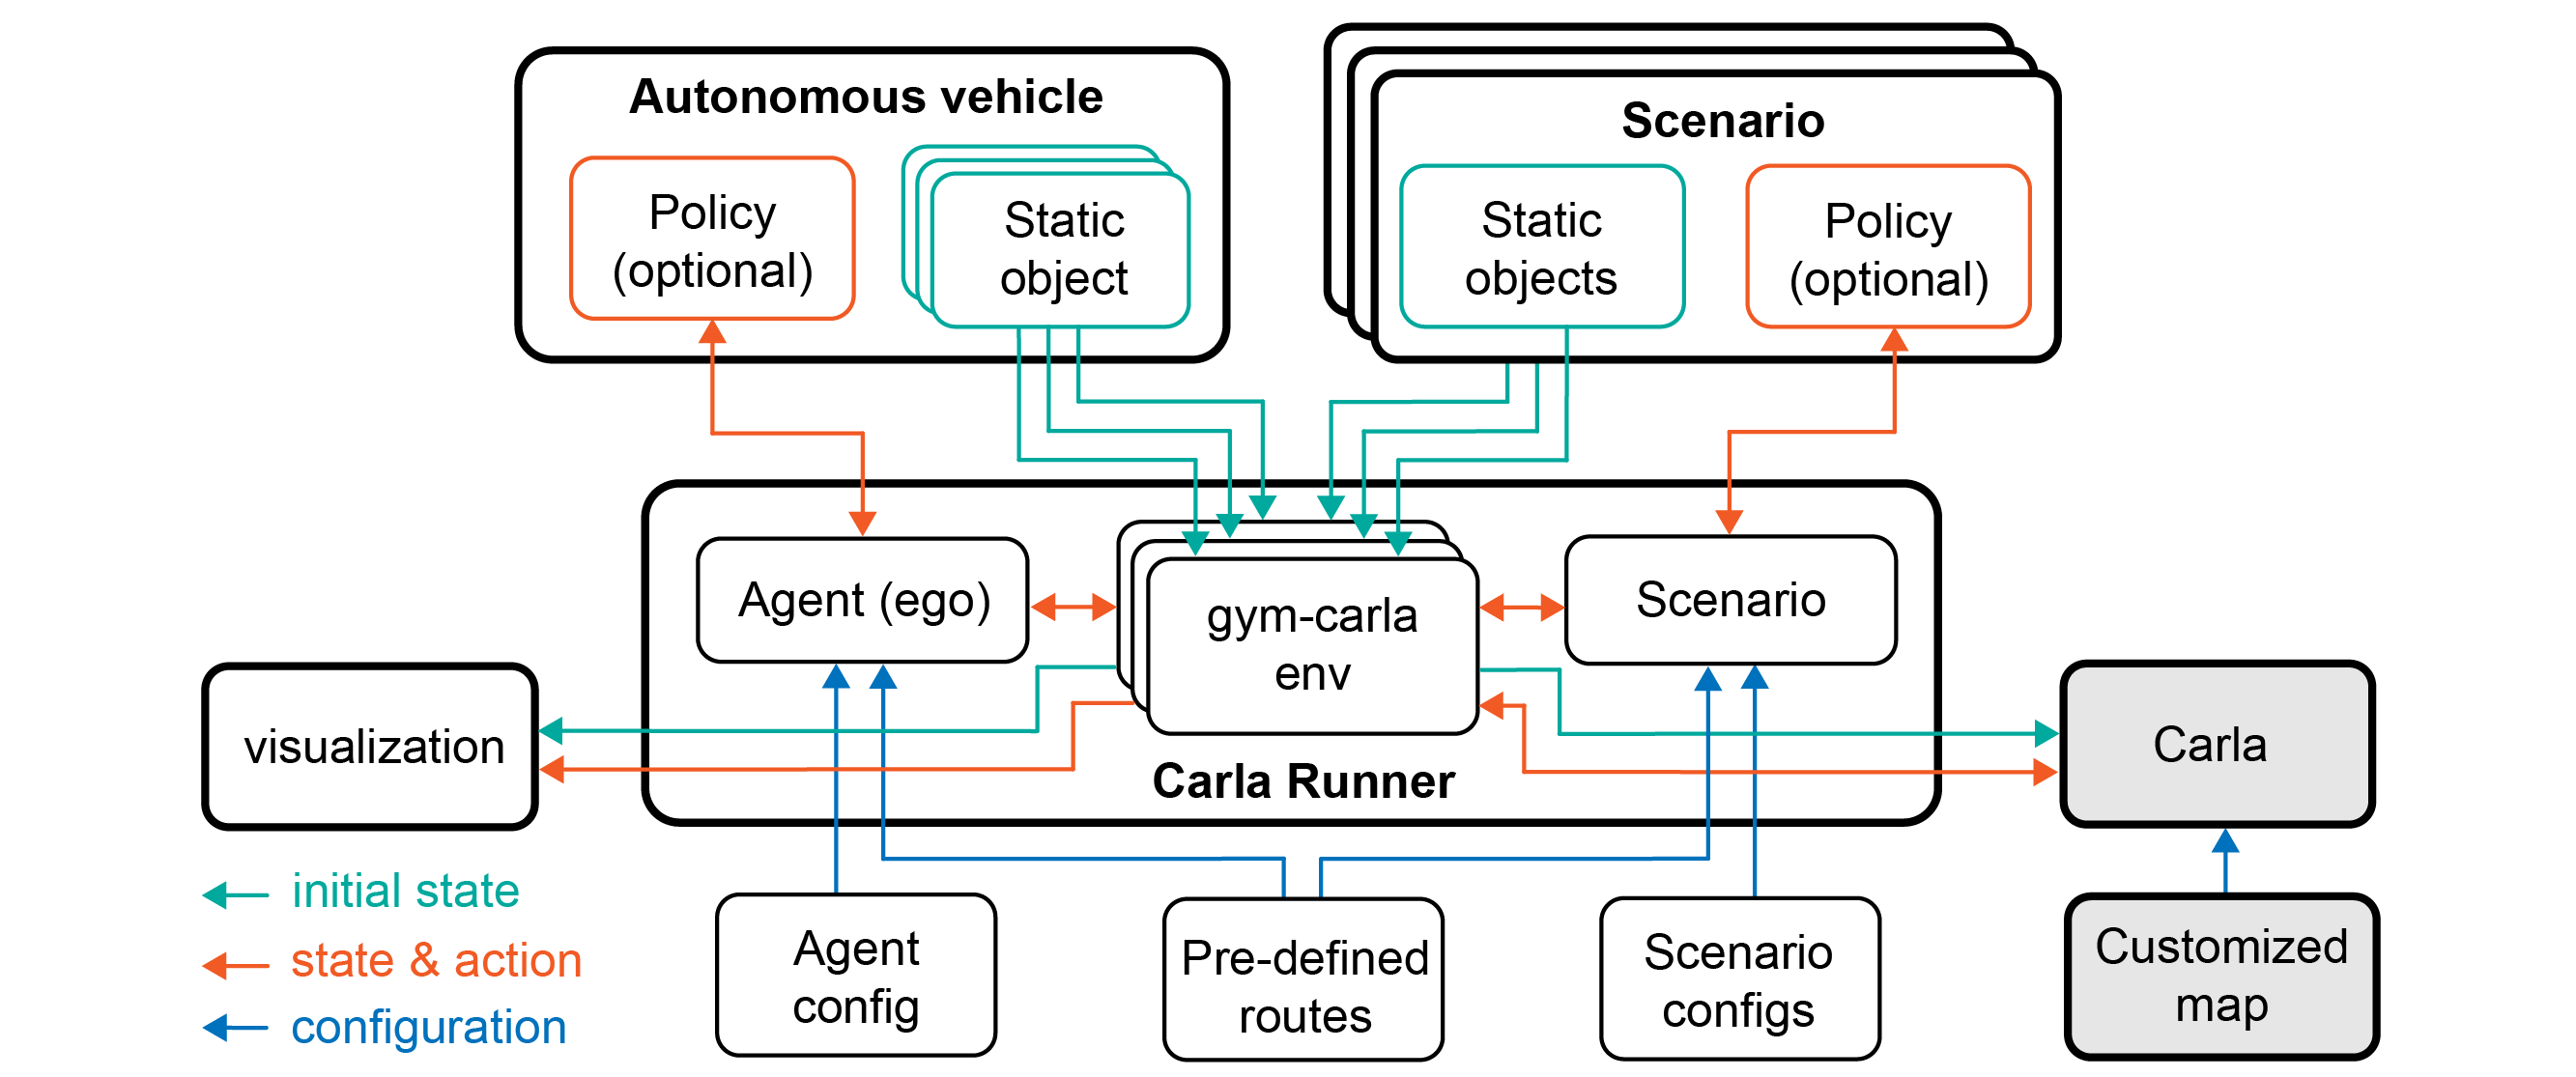
\includegraphics[width=1.0\textwidth]{"images/chatscene项目结构.pdf"}
	\caption{chatscene项目结构}
	\label{fig:chatscene_framework}
\end{figure}
然而,ChatScene 在以下方面存在一定局限:
\begin{itemize}
	\item \textbf{依赖检索}:ChatScene 无法自由生成未在数据库中存在的新场景,这限制了其在生成创新性场景方面的能力。
	\item \textbf{生成能力有限}:ChatScene 缺乏直接从自然语言生成代码的能力,这使得其在处理复杂的自然语言描述时存在困难。
	\item \textbf{多样性受限}:ChatScene 的生成结果受制于数据库的规模和覆盖范围,这限制了其生成场景的多样性和创新性。
\end{itemize}

为了克服这些局限,本项目在 ChatScene 的基础上进行了创新。我们引入了 GPT-4o 等大型语言模型,直接基于自然语言生成 Scenic 场景脚本。这种方法不仅解决了检索方法的局限性,还提升了场景的创新性与多样性。通过这种方式,我们能够生成更加复杂、多样化的场景,为高保真智能驾驶仿真系统构建提供了新的技术路径。此外,本项目还通过微调这些大模型,使其能够更好地适应智能驾驶场景生成的需求,从而进一步提高了生成场景的质量和可用性。